% !TeX root = ../document.tex
\documentclass[../document.tex]{subfiles}
\lstset{inputpath=sections}
\begin{document}

	\subsection{Polynomial regression}
	Linear models used so far are easy to interpret and if the true relationship is not approximately linear, limited in predictive power. So we increase the predictive power but want to maintaining as much interpretability as possible if we relax the linearity assumption.

	\paragraph{Extension to linear regression}
	We admit different powers of the original predictor variables as new predictor variables and then perform linear regression.
	\begin{equation}
	\begin{split}
		\text{let} \quad X_{k} &= X^{k}_1 \quad \text{for} \quad k>0\\
		Y &= \beta_{0} + \beta_{1}X_{1} + \beta_{2}X_{2} + \dots + \beta_{d}X_{d}\\
		&\Leftrightarrow  \\
		y_{i} &= \beta_{0}+\beta_{1}x_{i}+\beta_{2}x_{i}^2 + \dots + \beta_{d}x_{i}^d+\epsilon_{i} \\
	\end{split}
	\end{equation}
	By treating $X_1^k$ as a new predictor $X_k$, the model remains linear, allowing us to use it in regular linear regression.
	This also extends to classification problems:
	\begin{equation}
		Pr(y_{i}>250|x_{i})=\frac{exp(\beta_{0}+\beta_{1}x_{i}+\beta_{2}x_{i}^2+...+\beta_{d}x_{i}^d)}{1+exp(\beta_{0}+\beta_{1}x_{i}+\beta_{2}x_{i}^2+...+\beta_{d}x_{i}^d)}
	\end{equation}

	\textbf{Problem}: $\hat{y}$ is influenced by low and high $x_i$ predictors equally. $Y(x=1000)$ is equally important as $Y(x=0)$ for $\hat{y}(0)$. \\
	\textbf{Solution}: subdivide X into regions, turning $f^{*}(x)$ into a \textbf{step function}, with different weights per region.

	\subsection{Step functions}

	\paragraph{Local approximations}
	Step functions allow for local approximations by braking X into bins and fitting a different constant in each bin (stepwise uniform pdf $C_k$).
	\begin{center}
		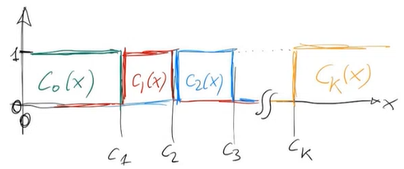
\includegraphics[width=.5\textwidth]{pictures/stepwise_function}
	\end{center}
	\begin{equation}
	\begin{split}
		&\hat{y}_{i}=\hat{\beta}_{0}+\hat{\beta}_{1}C_{1}(x_{i})+\hat{\beta}_{2}C_{2}(x_{i})+\dots+\hat{\beta}_{K}C_{K}(x_{i})+\epsilon_{i}\\
		&C_k(X) = \begin{cases}
			1 & \text{if } c_{k}<X < c_{k+1}\\
			0 & \text{otherwise} \\
		\end{cases} \\
		&C_{0}(X)+C_{1}(X)+\dots+C_{K}(X)=1 \qquad \text{(due to complementary ranges)}\\
		&\hat{\beta}_{k} = \text{ avg} (y) \text{ with } {c_{k}}<x<{c_{k+1}}
	\end{split}
	\end{equation}
	This function remains linear and can be used for classification problems:
	\begin{equation}
		Pr(y_{i}>250|x_{i})=\frac{exp(\beta_{0}+\beta_{1}C_{1}(x_{i})+\dots+\beta_{K}C_{K}(x_{i}))}{1+exp(\beta_{0}+\beta_{1}C_{1}(x_{i})+\dots+\beta_{K}C_{K}(x_{i}))}
	\end{equation}
	\textbf{Problem}: piecewise constant is a crude approximation.
	\textbf{Solution}:

	\subsection{Basis functions}

	\paragraph{A more general approach}
	Polynomial and piecewise-constant regression models are special cases of a basis function approach. Instead of fitting a linear model in X we fit a linear model in some basis functions \(b_{j}\)
	\begin{equation}
	\begin{split}
		&y_{i}=\beta_{0}+\beta_{1}b_{1}(x_{i})+\beta_{2}b_{2}(x_{i})+...+\beta_{K}b_{K}(x_{i})+\epsilon_{i}\\
		&\text{For polynomial regression:}\\
		&b_{j}(x_{i})=x_{i}^j\\
		&b_{j}(x_{i})=I(c_{j}\leq x_{i} < c_{j+1})
	\end{split}
	\end{equation}
	This is an elegant approach. We can use standard linear regression but applying it to the model having the original predictor values transformed by the basis functions. Hence all the inference tools for linear models are available for this non-linear fitting method.

	\subsection{Regression splines}

	\paragraph{Piecewise polynomial}
	Combining the local approach of step function and the flexibility of polynomials by fitting low degree polynomials over different regions of X.\\
	For example a cubic polynomial of the following form is fitted locally.
	\begin{equation}
	\begin{split}
		y_{i}&=\beta_{0}+\beta_{1}x_{i}+\beta_{2}x_{i}^2+\beta_{3}x_{i}^3+\epsilon_{i}\\
		y_{i}&=\begin{cases}
			\beta_{01}+\beta_{11}x_{i}+\beta_{21}x_{i}^2+\beta_{31}x_{i}^3+\epsilon_{i} \text{  if  } x_{i} < c\\
			\beta_{02}+\beta_{12}x_{i}+\beta_{22}x_{i}^2+\beta_{32}x_{i}^3+\epsilon_{i} \text{  if  } x_{i} \geq c
		\end{cases}
	\end{split}
	\end{equation}
	For example if there is a knot at c we have a cubic polynomial on the left and another one the right of c. Using more knots leads to more flexible fits.

	\paragraph{Constraints and splines}
	We would like the overall function to be continuos, with smooth transitions between polynomial functions. Hence we add the constraint, that at a knot both polynomials must have the same value (no jumps, can be done by tweaking offset $\beta_0$), the same slope (same 1. order derivatives) and the same rate of change (same 2. order derivative). These 3 constraints reduce the degrees of freedom by 1 each, leading to \textbf{+1 degree of freedom per knot}.

	\paragraph{The spline basis representation}
	How can we fit cubic splines to the data? The most elegant approach is based on the spline basis representation.
	\begin{equation}
		y_{i}=\beta_{0}+\beta_{1}b_{1}(x_{i})+\beta_{2}b_{2}(x_{i})+...+\beta_{K+3}b_{K+3}(x_{i})+\epsilon_{i}
	\end{equation}
	We use a truncated power function $h(x, \xi_k)$ as the basis function (previously $b_k$) for each knot, where $\xi_k$ is a knot.
	\begin{equation}
		h(x,\xi_k)=(x-\xi_k)_{+}^3=
		\begin{cases}
			(x-\xi_k)^3 \text{  if  } x > \xi_k\\
			0 \text{  otherwise  }
		\end{cases}
	\end{equation}
	One can show, that the following expression will have a discontinuity in only the third derivative at \(\xi_k\). In other words, the function will stay continuous and have continuous first and second derivatives.
	\begin{equation}
		y_{i}=\beta_{0}+\beta_{1}x_{i}+\beta_{2}x_{i}^2+\beta_{3}x_{i}^3 + \sum_{k=1}^{K}{\beta_{(k+3)}h(x_i,\xi_k)}+\epsilon_{i}
	\end{equation}
	Hence in order to fit a cubic spline to a data set using K knots we perform least squares regression with an intercept and 3+K predictors of the following form.
	\begin{equation}
		X, X^2, X^3, h(X,\xi_{1}),h(X,\xi_{2}),...,h(X,\xi_{K})
	\end{equation}

	\paragraph{Natural spline}
	As $x$ grows past the last knot (and prior to the first knot), the variance can grow rapidly. This can be improved by limiting the function to be linear for values $x<\xi_1$ and $\xi_k<x$. Doing so removes an additional 2 degrees of freedom at each end of the graph (2. \& 3. derivative = 0, -4 DoF total).

	\paragraph{Choosing the number ($K$) and locations of the knots ($\xi$)}
	The density of knots should reflect the amount of data so as to allow for enough flexibility where needed, without overfitting on sparse regions. For this, percentile markers can be used.\\
	For example using $K=3$ knots, we may place them at the $25^{th}$, $50^{th}$ and $75^{th}$ percentile. $K$ can be determined via cross validation.

	\paragraph{Comparison to polynomial regression}
	Regression splines are usually superior to polynomial regression. Regression splines can increase flexibility by adding knots, while polynomial regression needs to add powers of the predictor variable.

	\subsection{Smoothing splines}
	A smoothing spline $g(X)$ is a natural (linear at both ends) cubic spline with knots at every unique value of $x_{i}$ ($K=n$). This results in a spline with far too many degrees of freedom. As a counter-measure, we add a roughness cost the cost function $J(\beta)$. This penalizes roughness and limits the degrees of freedom. This also removes the need to manually pick sensible knots.
	\begin{equation}
	\begin{split}
		&y_{i}=\begin{cases}
			\beta_{01}+\beta_{11}x_{i}+\beta_{21}x_{i}^2+\beta_{31}x_{i}^3+\epsilon_{i} \text{  if  } x_{i} < c\\
			\beta_{02}+\beta_{12}x_{i}+\beta_{22}x_{i}^2+\beta_{32}x_{i}^3+\epsilon_{i} \text{  if  } x_{i} \geq c
		\end{cases}\\
		&RSS=\sum_{i=1}^{n}(y_{i}-g(x_{i}))^2\\
		&\text{Roughness} = \int g''(t)^2dt \qquad \begin{cases}
			=0 & \text{linear}\\
			\approx \infty & \text{very jagged}\\
		\end{cases}\\
		&J(\beta)=\sum_{i=1}^{n}(y_{i}-g(x_{i}))^2+\lambda\int g''(t)^2dt\\
		&LOOCV_{(n)}=\frac{1}{n}\sum_{i=1}^{n}(\frac{y_{i}-\hat{y}_{i}}{1-h_{i}})^2\\
	\end{split}
	\end{equation}

	\subsection{Local regression}

	\paragraph{Using local data for prediction}
	\begin{center}
		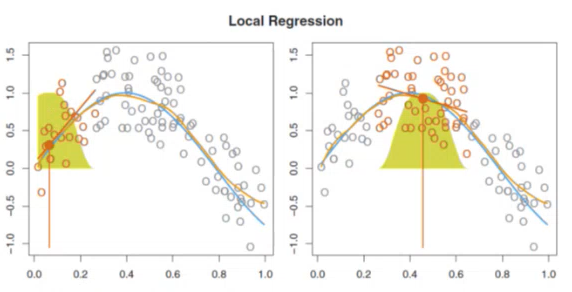
\includegraphics[width=.5\textwidth]{pictures/local_regression}
	\end{center}
	Local regression uses only data close to a target point \(x_{0}\) to fit a flexible non-linear function. Local regression has several parameters:
	\begin{itemize}
		\item Weighting function \(K(x_{i},x_{0})\)
		\item degree of the polynomial fit
		\item span s which defines how many training points are used for the local fit
	\end{itemize}
	The most important choice is the span s. The smaller the value of s, the more local the fit is and hence the more flexible the function becomes. Again, cross-validation is used for finding the best value for the span s.

	\sectionbreak
	\subsection{Generalized additive models}
	All methods of this chapter have been developed for a single predictor. Generalized additive models (GAMs) extends these ideas to multiple predictors.

	\paragraph{GAMs for regression problems}
	Recall the multiple regression model.
	\begin{equation}
		y_{i}=\beta_{0}+\beta_{1}x_{i1}+\beta_{2}x_{i2}+...+\beta_{p}x_{ip}+\epsilon_{i}
	\end{equation}
	The obvious extension of this formula is by replacing the linear components \(\beta_{j}x_{ij}\) with a smooth non-linear function \(f_{j}(x_{ij})\), resulting in the new model.
	\begin{equation}
		y_{i}=\beta_{0}+\sum_{j=1}^{p}f_{j}(x_{ij})+\epsilon_{i} = \beta_{0}+f_{1}(x_{i1})+f_{2}(x_{i2})+...+f_{p}(x_{ip})+\epsilon_{i}
	\end{equation}
	This is an example of a GAM. It is called an additive model because we calculate a separate \(f_{j}\) for each \(X_{j}\) and then add together all of their contributions.

	\paragraph{Pros and cons of GAMs}
	Pros of GAMs
	\begin{itemize}
		\item GAMs allow us to fit a non-linear \(f_{j}\) for each \(X_{j}\), so that we can automatically model non-linear relationships that standard linear regression will miss. This means that we do not need to manually try out many different transformations on each variable individually.
		\item The non-linear fits can potentially make more accurate predictions for the response Y.
		\item Because the model is additive, we can still examine the effect of each \(X_{j}\) on > individually while holding all of the other variables fixed. Hence if we are interested in inference, GAMs provide a useful representation.
	\end{itemize}
	The main negative aspect is that the model is restricted to be additive. With many variables, important interactions can be missed. However, as with linear regression, we can manually add interaction terms to the GAM model.

	\paragraph{GAMs for classification problems}
	GAMs are also useful, if the responses are qualitative.
	\begin{equation}
		log(\frac{p(X)}{1-p(X)})=\beta_{0}+f_{1}(X_{1})+f_{2}(X_{2})+...+f_{p}(X_{p})
	\end{equation}
	For simplicity, we assume the response is either 1 or 0.
\end{document}
